\chapter{Stakeholder Analysis} \label{ch:Stakeholder Analysis}

\begin{figure}[h]
    \centering
    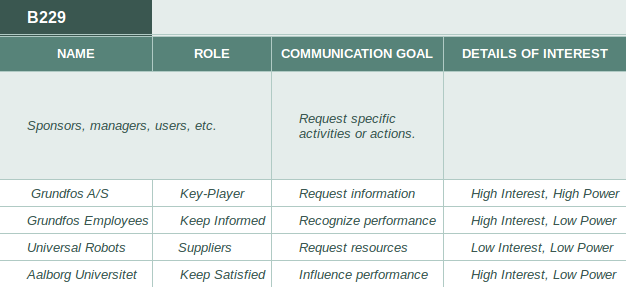
\includegraphics[scale=0.65]{StakeholderAnalysis/Stakeholder.png}
    \caption{Stakeholder Analysis} 
    \label{fig:Stakeholder} 
\end{figure}

\section{Grundfos A/S}\label{ch:grundfosas-stake}
Grundfos A/S are stakeholders with high interest and high power, as they are financing and producing the robot. Their interest is high, because the development of the robot might have a direct impact on the company. The development would be very hard without funding, which also gives Grundfos a lot of power. 



\section{Grundfos Employees}\label{ch:grundfosemp-stake}
Employees of Grundfos are stakeholders, who have a high interest, but a low influence.\\ The reason for this is they have no final say in whether the solution should be implemented. The Employees may have to learn new skills, or move to new workstations for the reason, that the new robot solution might be taking over the production station, which the employee was working at before.


\section{Universal Robots}\label{ch:Universalrobots-stake}
The suppliers of the robotic manipulator in this case has a low interest and a low power, this is because they do not have any say in the matter, if it such be they manipulator or if it is a competitors manipulator, they can adjust the prizes on the manipulator so we will choose their product for the this case. 


\section{Aalborg University}\label{ch:Aau-stake}
Aalborg University has a great interest in the development of robotics from a research and information perspective. For this reason they may have interest in investing in further development and improvement of a technology such as the UR. 